\documentclass{article}

\usepackage{booktabs} % for better table formatting
\usepackage{siunitx} % for aligning table columns by decimal point
\usepackage{graphicx}
\usepackage{pgfplots} % for generating charts
\usepackage{tikz} % for drawing graphics


\begin{document}

\title{\vspace{-3cm}CSCI 4320 Assignment 4 Report}
\author{Zhiqi Wang wangz56@rpi.edu}
\date{\today}
\maketitle

Here are the result from the experiments with local GPU reduction and global CPU reduction:

\begin{table}[h!]
  \centering
  \begin{tabular}{|c|c|c|}
  \hline
  \textbf{GPU Configuration} & \textbf{O3 Flag} & \textbf{Runtime (s)} \\ \hline
  6 GPUs & Enabled & 1.2927 \\ \hline
  12 GPUs & Enabled & 0.8923 \\ \hline
  24 GPUs & Enabled & 0.7151 \\ \hline
  48 GPUs & Enabled & 0.5447 \\ \hline
  6 GPUs & Disabled & 3.2824 \\ \hline
  12 GPUs & Disabled & 1.8033 \\ \hline
  24 GPUs & Disabled & 1.1289 \\ \hline
  48 GPUs & Disabled & 0.8062 \\ \hline
  \end{tabular}
  \caption{GPU Runtimes with and without O3 flag}
  \end{table}
  
  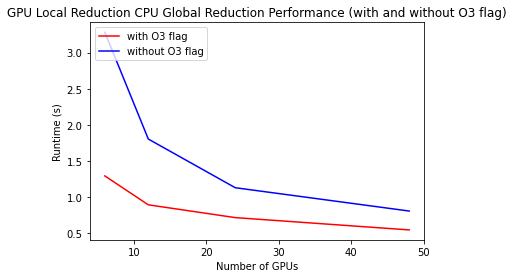
\includegraphics[width=\textwidth]{gpu_local.png}
  

  \begin{table}[h!]
  \centering
  \begin{tabular}{|c|c|c|}
  \hline
  \textbf{CPU Configuration} & \textbf{O3 Flag} & \textbf{Runtime (s)} \\ \hline
  32 ranks & Enabled & 0.4813 \\ \hline
  64 ranks & Enabled & 0.2984 \\ \hline
  128 ranks & Enabled & 0.1247 \\ \hline
  256 ranks & Enabled & 0.0865 \\ \hline
  32 ranks & Disabled & 0.4848 \\ \hline
  64 ranks & Disabled & 0.3266 \\ \hline
  128 ranks & Disabled & 0.0143 \\ \hline
  256 ranks & Disabled & 0.0671 \\ \hline
  \end{tabular}
  \caption{CPU Runtimes with and without O3 flag}
  \end{table}

  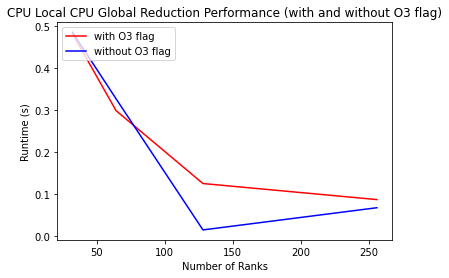
\includegraphics[width=\textwidth]{cpu_local.png}

\begin{itemize}

  \item Speedup with O3 flag:
  For GPU with O3 flag, the average speed up is:

    \begin{itemize}
    \item 6 GPUs: $\frac{3.2824s}{1.2927s}=2.54x$ faster
    \item 12 GPUs: $\frac{1.8033s}{0.8923s}=2.02x$ faster
    \item 24 GPUs: $\frac{1.1289s}{0.7151s}=1.58x$ faster
    \item 48 GPUs: $\frac{0.8062s}{0.5447s}=1.48x$ faster
    \end{itemize}

    For CPU with O3 flag, the average speed up is:

    \begin{itemize}
    \item 32 ranks: $\frac{0.4848s}{0.4813s}=1.007x$ faster
    \item 64 ranks: $\frac{0.3266s}{0.2984s}=1.094x$ faster
    \item 128 ranks: $\frac{0.0143s}{0.1247s}=0.114x$ slower
    \item 256 ranks: $\frac{0.0671s}{0.0865s}=0.776x$ slower
    \end{itemize}
  
  \item maximum speedup across all cases relative to using a single compute-node using 32 MPI in total:
  \begin{itemize}
    \item Maximum speedup relative to using 6 GPUs:
    \begin{itemize}
    \item 48 GPUs: $\frac{3.2824s}{0.5447s}=6.04x$ faster
    \end{itemize}
    \item Maximum speedup relative to using 32 MPI ranks:
    \begin{itemize}
    \item 256 ranks: $\frac{0.4848s}{0.0865s}=5.60x$ faster
    \end{itemize}
    \end{itemize}

  \item Did GPUs always outperform the CPU cases. Why or why not for your code?\\
  No, in fact, CPU always outperforms GPU. I think this is because it's not a fair comparison: First, this is not a large enough test for GPU to show it's ability, since it's not large enough and GPU takes time to initialize the CUDA, CPU performs better. Second, GPU and CPU here is not comparing in the same scale, we used at most 48 GPUs but we used 256 ranks of CPU. I can't say which configuration is better. Third, our \texttt{reduce7} only reduce to an array of sum, we still need to calculate further to get the local sum by cpu addition with for loop. Fourth, \texttt{MPI\_Reduce} with \texttt{MPI\_Sum} might be better optimized for this task. In conclusion, for this case, I would prefer CPU over GPU simply because it's faster. 

  \item Finally, explain why you think FASTEST configuration was faster than others.\\
  My fastest configuration is 128 ranks without O3 flag. This configuration being the fastest doesn't mean it's always the fastest, since the task not not large enough for 128 ranks and above to see the difference. My guess for 128 ranks being faster than 256 ranks is because the more ranks we use, the more time it takes to initialize the MPI, and the more time it takes to communicate between ranks. Therefore, 128 ranks is the fastest configuration for this size of task.

\end{itemize}

\end{document}